% TeX'ing this file requires that you have AMS-LaTeX 2.0 installed
% as well as the rest of the prerequisites for REVTeX 4.0
%
% See the REVTeX 4 README file
% It also requires running BibTeX. The commands are as follows:
%
%  1)  latex apssamp.tex
%  2)  bibtex apssamp
%  3)  latex apssamp.tex
%  4)  latex apssamp.tex
%
%\documentclass[prb,showkeys,preprintnumbers,amsmath,amssymb, 11pt]{revtex4}
%\documentclass[preprint,showpacs,showkeys,preprintnumbers,amsmath,amssymb]{revtex4}

% Some other (several out of many) possibilities
%\documentclass[preprint,aps]{revtex4}
%\documentclass[aps, two column, amsmath,amssymb,floatfix]{revtex4}
%\documentclass[showkeys,showpacs,amsmath,amssymb,onecolumn,superscriptaddress,prl]{revtex4-1}% Physical Review B  
\documentclass[aps,prl,reprint,showpacs,floatfix,superscriptaddress, onecolumn]{revtex4-2}

\usepackage{amsmath,amsthm,amssymb}
\usepackage{graphicx}% Include figure files
\usepackage{dcolumn}% Align table columns on decimal point
\usepackage{bm}% bold math
\usepackage{color}
\usepackage{epsfig}
\usepackage{multirow}
\usepackage{mathrsfs}
\usepackage{hyperref}
\usepackage{cleveref}
\usepackage{epstopdf}
\usepackage{subfigure}
\usepackage{autobreak}

%Macros for mathematical notations

\newcommand{\V}[1]{\boldsymbol{#1}} %# vector
\newcommand{\M}[1]{\boldsymbol{#1}} %# matrix
\newcommand{\Set}[1]{\mathbb{#1}} %# set
\newcommand{\D}[1]{\Delta#1} %# \D{t} for time step size
\renewcommand{\d}[1]{\delta#1} %# \d{t} for small increment
\newcommand{\norm}[1]{\left\Vert #1\right\Vert } % norm
\newcommand{\abs}[1]{\left|#1\right|} %abs

\newcommand{\grad}{\M{\nabla}} %gradient
\newcommand{\av}[1]{\left\langle #1\right\rangle } %take average

\newcommand{\sM}[1]{\M{\mathcal{#1}}} %matrix in mathcal font
\newcommand{\dprime}{\prime\prime} % double prime
%\global\long\def\i{\iota}
%\renewcommand{\i}{\iota} %i for imaginary unit
%\renewcommand{\i}{\mathsf i} %i for imaginary unit
\newcommand{\follows}{\quad\Rightarrow\quad} %=>
\newcommand{\eqd}{\overset{d}{=}} %=^d
\newcommand{\spe}[1]{\mathscr{#1}}  %important quantities in mathscr font
\newcommand{\eps}{\epsilon}

\usepackage{algorithm}
\usepackage{algorithmic}



\begin{document}
\preprint{Preprint}

\title{Supplementary Information}
\author{Xuanzhao Gao}
\email{xz.gao@connect.ust.hk}
\affiliation{Thrust of Advanced Materials, The Hong Kong University of Science and Technology (Guangzhou), Guangdong, China}
\affiliation{Department of Physics, The Hong Kong University of Science and Technology, Hong Kong SAR, China}

\author{Zecheng Gan} \thanks{Corresponding author}
\email{zechenggan@ust.hk}
\affiliation{Thrust of Advanced Materials, The Hong Kong University of Science and Technology (Guangzhou), Guangdong, China}
\affiliation{Department of Mathematics, The Hong Kong University of Science and Technology, Hong Kong SAR, China}

\maketitle

\section{Solution to the Green's function}

In main text, we write the Green's function of the system as
\begin{equation}
    -\grad\cdot\left[\eta(\V r) \grad G(\V{r},\V{s})\right] = 4 \pi \d(\V r - \V s )\;,\label{eq:Green4Poisson}
\end{equation}
where~$z_s \in [0, L_z]$ because of the confinement, so that Eq.~\eqref{eq:Green4Poisson} can be transformed into
\begin{equation}\label{eq:Green_sim}
    - \grad^2 G(\V{r},\V{s}) = 4 \pi \d(\V r - \V s ),~z_s \in (0, L_z)\;,\\
\end{equation}
together with continuity of~$G(\V r, \V s)$ and~$\eta(\V{r}) \partial_z G(\V r, \V s)$ at~$z = 0$ and~$L_z$ as boundary conditions.
According to the symmetry of the system, we apply separation of variables to both side of Eq.~\eqref{eq:Green_sim} via plane wave expansion using similar method as the one used by Levin~\cite{dos2017simulations}, given by
\begin{equation} \label{eq:single_G}
    - \grad^2 G(\V{r},\V{s}) = \frac{1}{\pi} \grad^2 \iint_{-\infty}^{+\infty} g(k, z, z_s) e^{i \V{k} \cdot \V{\rho}} \text{d}k_x \text{d} k_y = 4 \pi \frac{1}{(2 \pi)^2} \delta(z - z_s) \iint_{-\infty}^{+\infty} e^{i \V{k} \cdot \V{\rho}} \text{d}k_x \text{d} k_y\;,
\end{equation}
so that when~$k > 0$,~$g(k, z, z_s)$ satisfy ODE and Robin boundary conditions given by
    \begin{gather}\label{eq:g_ODE}
        \frac{\partial^2 g(k, z, z_s)}{\partial z ^2} - k^2 g(k, z, z_s) = \delta(z - z_s)\;,\\
        \eps \partial_z g(k, L_z, z_s) + \eps_1 k g(k, L_z, z_s) = \eps \partial_z g(k, 0, z_s) - \eps_2 k g(k, 0, z_s) = 0\;.
    \end{gather}
As already shown in main text, the solution of Eq.~\eqref{eq:g_ODE} is
\begin{equation}\label{eq:g_solution}
    g(k, z, z_s) = \frac{1}{2k} \frac{1}{\gamma_1 \gamma_2 \exp{(-2 k L_z)} - 1} \sum_{i = 1}^{4} \Gamma_l \text{e}^{-k a_l}\;,
\end{equation}
where~$\Gamma_l = \left[1, ~\gamma_1, ~\gamma_2, ~\gamma_1 \gamma_2 \right]$ and~$a_l = [\abs{z - z_s}, ~z + z_s, ~2L_z - (z + z_s), ~2L_z - \abs{z - z_s}]$.
However, Eq.~\eqref{eq:g_solution} diverges as $k\to 0$ so that the 0-th mode needs to be treated carefully.
Physically, it corresponds to proposing the proper FBC as $z\to\pm\infty$ so that the divergent image charge series (as depicted in Fig.~1 in main text) can be renormalized.
For $k = 0$, it is understood that the electric field should be a function of~$z$ only, hence~$\hat E_{k \to 0}(z \to +\infty)$ and $\hat E_{k \to 0}(z \to -\infty)$ are both constants to satisfy Gauss's law.
The divergence issue thus can be properly renormalized, which leads us to
\begin{equation}\label{eq:g_k=0}
    g(k = 0, z, z_s) = - \frac{\abs{z - z_s}}{2}.
\end{equation}
Thus~$g(k, z, z_s)$ is fully solved.

\section{Detailed Derivations for Quasi Ewald method}

To handle the long range nature of electrostatic interaction, we apply strategy similar to Ewald splitting in our method, by dividing the Dirac delta function into two parts, given by
\begin{equation}\label{eq:split}
    \delta(\V r) = \left[\d(\V r) - \frac{\alpha}{\pi} e^{-\alpha \rho^2}\d(z)\right] + \frac{\alpha}{\pi} e^{-\alpha \rho^2}\d(z)\;,
\end{equation}
with~$\V{\rho} = (x, y)$,~$\rho = \sqrt{x^2+y^2}$, and the choice of $\alpha$ will be determined by considerations of computational efficiency.
Subtracting and adding the Gaussian term split the delta charge density into two terms, so that the calculation converge more rapidly in both real and reciprocal spaces.
It also avoids the subtle situation of the Gaussian charge cloud overlapping the substrates.
Due to the splitting strategy Eq.~\eqref{eq:split}, the doubly periodic Green's function can be decomposed into short- and long-range components, i.e., $G_1$ and $G_2$, given by
\begin{equation} \label{eq:G12}
    \begin{split}
        -\grad^2 G_1(\V r, \V s) &= 4 \pi \sum_{\V{m}} \left[\d(\V r - \V s_m) - \frac{\alpha}{\pi} \d(z - z_s) e^{-\alpha \Delta \rho_{\V{m}}^2} \right]\;,\\
    	-\grad^2 G_2(\V r, \V s) &= 4 \pi \sum_{\V{m}} \frac{\alpha}{\pi} \d(z - z_s) e^{-\alpha \Delta \rho_{\V{m}}^2}\;,
    \end{split}
\end{equation}
where~$\V{m} = (m_x, m_y) \in \mathbb{Z}^2$ is the index of doubly periodic images.
Then by similar method used in Eq.~\eqref{eq:single_G}, we can have
\begin{equation}\label{eq:G12_int}
    \begin{split}
        G_1(\V r, \V s)
        = & - \sum_{\V{m}} \int_{0}^{+\infty} 2 g(k, z, z_s) (1-e^{-\frac{\V{k}^2}{4 \alpha}}) J_0(k \Delta \rho_m) k \text{d} k \;, \\
        G_2(\V r, \V s)
        = & - \frac{4 \pi}{L_x L_y} \sum_{\V{k}} g(k, z, z_s) e^{-\frac{\V{k}^2}{4 \alpha}}e^{\mathrm{i} \V{k} \cdot \Delta \V \rho_m}\;,
    \end{split}
\end{equation}
where~$g(k, z, z_s)$ is already given by Eq.~\eqref{eq:g_solution}, and they decay rapidly in real and reciprocal space, respectively.
So that we can choose cutoff in real and reciprocal space, i.e.,~$r_c$ and~$k_c$ to transform summations into finite ones, given by
\begin{equation}
    \sum_{\V m} \to \sum_{\Delta \rho < r_c},~\sum_{\V{k}} \to \sum_{k < k_c}\;.
\end{equation}
In our problem, we choose 
\begin{equation}
    r_c = \frac{s}{\sqrt{\alpha}},~k_c = 2 s \sqrt{\alpha}\;,
\end{equation}
where~$s$ is a parameter to control the error, so that $r_c k_c = C$ and calculation in real and reciprocal space will have similar accuracy.

\section{Numerical calculation of Cauchy principal value}

As mentioned in main text, if~$\gamma_1 \gamma_2 > 1$, we need to calculate Cauchy principal value given by
\begin{equation}
    I = \text{p.v.} \left[ \int_0^{\infty} \frac{f(k)}{\exp{\left[-2 L_z (k - k_0)\right]} - 1} \text{d}k \right]\;,
\end{equation}
where~$f(k)$ is a non-divergent part of the integrand and~$k_0 = \ln{(\gamma_1 \gamma_2)} / 2L_z$.
Here we consider neighbourhood of the divergent point $k_0$, i.e.~$\left(k_0 - \delta, k_0 + \delta \right)$, where the integral can be rewritten as
\begin{equation}\label{eq:I_d}
    I_{\delta} = \int_{-\delta}^{\delta} \frac{f(k' + k_0)}{e^{-2k' L_z} - 1} \text{d} k' = \int_{-\delta}^{\delta} \left( f(k_0) + f'(k_0)k' + O(k^{\prime 2}) \right) \left( - \frac{1}{2 L_z k'} + E(k') \right) \text{d} k'\;,
\end{equation}
where
\begin{equation}
    E(k') = \frac{0.5 + \sum_{n = 0} {(-2L_z k')^{n + 1}} / {(n + 3)!}}{-1 + L_zk' - \sum_{n = 0} {(-2 L_z k')^{n + 2}} / {(n + 3)!}} = \frac{1}{e^{-2L_z k'} - 1} + \frac{1}{2 L_z k'}\;,
\end{equation}
is the expansion form at~$k' = 0$, which is a smooth function.
So that~$I_{\delta}$ can be further transformed as
\begin{equation}\label{eq:int_form}
    I_{\delta} = \int_{-\delta}^{\delta} \left[ - \frac{f(k_0)}{2 L_z k'} -  \frac{f'(k_0)}{2 L_z} + f(k_0)E(k') + O(k') \right] \text{d}k' = \int_{-\delta}^{\delta} f(k_0)E(k') \text{d}k' - \frac{f'(k_0) \delta}{L_z} + O(\delta^3)\;.
\end{equation}
In this way, the divergent part of the integral is properly handled numerically, which leads to
\begin{equation}\label{eq:}
    I = \left( \int_0^{k_0 - \delta} + \int_{k_0 + \delta}^{2 k_0} \right) g(k) \text{d} k + I_{\delta} + \int_{2 k_0}^{+\infty} f(k) \text{d} k\;,
\end{equation}
where 
\begin{equation}
    g(k) = \frac{f(k)}{\exp{\left[-2 L_z (k - k_0)\right]} - 1} + \frac{f(k_0)}{2 L_z (k - k_0)}\;.
\end{equation}
Reason of using~$g(k)$ rather than the original integrand in calculation is that~$(k - k_0)^{-1}$ part still has a scale of~$\delta^{-1}$ at~$k_0 \pm \delta$, which is still too large for calculation, directly removing it can further improve the accuracy.

For~$\gamma_1 \gamma_2 = 1$ case, the strategy above can not be applied directly because the principal value does not exits.
However, at the divergent point~$k_0 = 0$ we have
\begin{equation}
    \lim_{k \to k_0}  \frac{f(k)}{\exp{\left(-2 L_z k \right)} - 1} = \frac{1}{k_0} \sum_{l = 1}^4 \Gamma_l \;,
\end{equation}
which is a position independent variable and can be directly removed from the integral, so that we can integrate over
\begin{equation}
     \frac{f(k)}{\exp{\left(-2 L_z k \right)} - 1} + \frac{f(0) e^{-2 k L_z}}{2 L_z k}\;
\end{equation}
instead, where the later function is fast decaying and is position irrelevant.
Then Eq.~\eqref{eq:I_d} should be transformed as
\begin{equation}
    I_{\delta} = \int_{0}^{\delta} \frac{f(k')}{e^{-2k' L_z} - 1} \text{d} k' + \int_{0}^{\delta} \frac{f(0) e^{-2 k' L_z}}{2 L_z k'} \text{d} k' = \int_{0}^{\delta} \left( f(0) E(k')  - \frac{f'(0)}{2 L_z} + O(k^{\prime})\right) \text{d} k'\;,
\end{equation}
and the rest part can be calculated using the same method for~$k_0 > 0$ cases.


\section{Optimal Quadrature Scheme and Truncation Error Analysis}
Calculating the short-range component~$G_1$ is non-trivial. Especially, comparing with $\mathrm{erfc}(\cdot)$ for Ewald3D which is simple to evaluate accurately. In what follows, we discuss the details of our optimal quadrature scheme and its error analysis.

As shown in Eq.~\eqref{eq:G12_int}, to calculate~$G_1$ numerically we need to calculate the following integrals
\begin{equation}\label{eq:G_1_int}
\begin{split}
    I &= \int_{0}^{+\infty} g(k, z, z_s) \left( 1-e^{-\frac{\V{k}^2}{4 \alpha}} \right) J_0(k \Delta \rho) k \text{d} k\;\\
    & = \int_{0}^{+\infty} \frac{1}{2 (\gamma_1 \gamma_2 e^{-2k L_z} - 1)} \sum_{l = 1}^{4} \Gamma_l e^{-k a_l} \left( 1-e^{-\frac{\V{k}^2}{4 \alpha}} \right) J_0(k \Delta \rho) d k\;\\
    & = \int_{0}^{+\infty} \frac{1}{2 (\gamma_1 \gamma_2 e^{-2k L_z} - 1)} \sum_{l = 1}^{4} \Gamma_l e^{-k a_l} J_0(k \Delta \rho) d k - \int_{0}^{+\infty} \frac{1}{2 (\gamma_1 \gamma_2 e^{-2k L_z} - 1)} \sum_{l = 1}^{4} \Gamma_l e^{-k a_l -\frac{\V{k}^2}{4 \alpha}} J_0(k \Delta \rho) d k \;\\
    & = I_1 + I_2\;,
\end{split}
\end{equation}
where~$a_l \ge 0$, and~$\Gamma_l$ are constants as given in the main text.

All terms in the integrand of~$I_2$ are coupled with the factor~$\exp{\left(- k^2 / (4 \alpha)\right)}$, so that decay rapidly

For~$I_1$, using the fact that
\begin{equation}\label{eq:beta_split}
    \frac{1}{\gamma_1 \gamma_2 e^{-2k L_z} - 1} = \frac{\gamma_1 \gamma_2 e^{-2k L_z}}{\gamma_1 \gamma_2 e^{-2k L_z} - 1} - 1\;.
\end{equation}
and split Eq.~\eqref{eq:g_solution} into two parts as
\begin{equation}
    \begin{split}
        g_a(k, z, z_s) &= - \frac{1}{2k} \sum_{l = 1}^{4} \Gamma_l e^{-k a_l}\;,\\
        g_b(k, z, z_s) &= \frac{1}{2k} \frac{\gamma_1 \gamma_2}{\gamma_1 \gamma_2 e^{-2k L_z} - 1} \sum_{l = 1}^{4} \Gamma_l e^{-k (a_l + 2 L_z)}\;,
    \end{split}
\end{equation}
so that~$I_1 $ can also be divided into two parts, $ I_{1a} $ and $ I_{1b}$.
Notice that 
\begin{equation}
    \int_0^{\infty} e^{- k a}J_0(k \rho) dk = \frac{1}{\sqrt{a^2 + \rho^2}}\;,
\end{equation}
so that~$I_{1a}$ can be given analytically as
\begin{equation}
    I_{1a} = - \int_{0}^{+\infty} \frac{1}{2} \sum_{l = 1}^{4} \Gamma_l e^{-k a_l} J_0(k \Delta \rho) d k = - \sum_{l = 1}^{4} \frac{\Gamma_l}{2 \sqrt{a_l^2 + \Delta \rho^2}}\;.
\end{equation}

We still have to handle two infinite integrals, given by
\begin{equation}
    \begin{split}
        I_{1b} &= \int_{0}^{+\infty} \frac{1}{2 (\gamma_1 \gamma_2 e^{-2k L_z} - 1)} \sum_{l = 1}^{4} \Gamma_l e^{-k a_l -2 k L_z} J_0(k \Delta \rho) \text{d} k\;,\\
        I_2 &= - \int_{0}^{+\infty} \frac{1}{2 (\gamma_1 \gamma_2 e^{-2k L_z} - 1)} \sum_{l = 1}^{4} \Gamma_l e^{-k a_l -\frac{\V{k}^2}{4 \alpha}} J_0(k \Delta \rho) \text{d} k\;.
    \end{split}
\end{equation}

For both cases the integrands are coupled with fast decay factors,~$\exp{(-2 k L_z)}$ or~$\exp{\left[-k^2 / (4 \alpha)\right]}$, so that converge rapidly.
The denominator is also a function of~$k$, and its value under different~$\gamma_1 \gamma_2$ is shown in~Fig.~\ref{fig:beta}.
When~$\gamma_1 \gamma_2 < 1$, it has no zero-points on positive real axis, and its value is bounded near~$-1$, so that it can be directly calculated along the positive real axis on interval~$(0, +\infty)$.
When~$\gamma_1 \gamma_2 \geq 1$, it has a zero-point~$k_0 > 0$, so that we will have to use the strategy given by Eq.~\eqref{eq:int_form} and split it into integrals on~$(0, k_0 - \delta)$,~$(k_0 + \delta, k_0)$, and~$(2 k_0, +\infty)$.
The finite integrals can be directly calculated.
Traditionally, the infinite integrals can be calculated by Gauss–Laguerre quadrature or Gauss–Hermite quadrature.
However, recent work~\cite{trefethen2022exactness} has shown that evaluating such improper integrals via truncating them onto finite domains~$(0,~k_f)$ or~$(2k_0,~k_f)$ will lead to a better accuracy when using the same number of sampling points, simply because the integral on~$(k_f, \infty)$ is negligible.

\begin{figure}[htbp]
    \centering
    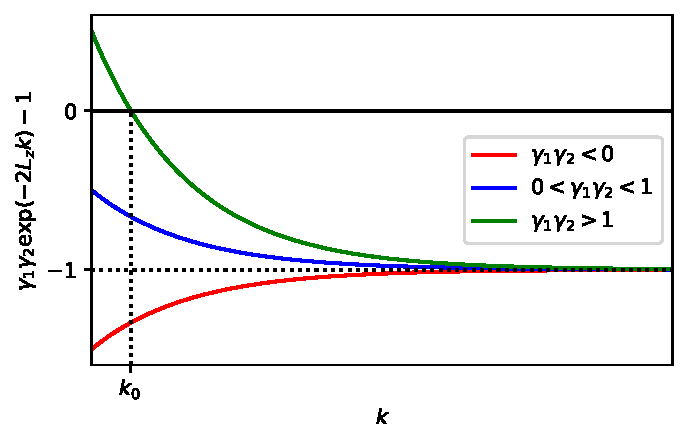
\includegraphics[width = 0.6 \linewidth]{SIfig/beta.pdf}
    \caption{The denominator of~$g_1(k, z, z_s)$ for different~$\gamma_1 \gamma_2$.}
    \label{fig:beta}
\end{figure}

On~$(k_f, +\infty)$, the minimum of~$\abs{\gamma_1 \gamma_2 e^{-2k L_z} - 1}$ can be given by
\begin{equation}
    \min{\abs{\gamma_1 \gamma_2 e^{-2k L_z} - 1}} = \min{\left\{1, \abs{\gamma_1 \gamma_2 e^{-2k_f L_z} - 1}\right\}} = \beta\;,
\end{equation}
so that the error on~$(k_f, \infty)$ is proportional to
\begin{equation}
    \begin{split}
        \Delta_{1b} &\propto \abs{\int_{k_f}^{+\infty} \frac{\sum_{l = 1}^{4} \Gamma_l e^{-k (a_l + 2 L_z)} J_0(k \Delta \rho)}{\gamma_1 \gamma_2 e^{-2k L_z} - 1}   \text{d} k} < \int_{k_f}^{+\infty} \sum_{l = 1}^{4} \abs{\Gamma_l} \beta^{-1} e^{ - 2k L_z} (k \Delta \rho)^{-0.5} \text{d} k = \chi_1 \text{erfc} \left( \sqrt{2 k_f L_z} \right)\;,\\
        \Delta_2 &\propto \abs{\int_{k_f}^{+\infty} \frac{\sum_{l = 1}^{4} \Gamma_l e^{-k a_l - k^2 / (4 \alpha)} J_0(k \Delta \rho)}{\gamma_1 \gamma_2 e^{-2k L_z} - 1}   \text{d} k} < \int_{k_f}^{+\infty} \sum_{l = 1}^{4} \abs{\Gamma_l} \beta^{-1} e^{ - k^2 / (4 \alpha)} \text{d} k = \chi_2 \mathrm{erfc}\left(\frac{k_{f}}{2 \alpha}\right)\;,
    \end{split}
\end{equation}
where~$\mathrm{erfc}(\cdot)$ is the error function and decay rapidly to~$0$.
Then all the integrals are over smooth functions on finite region, so that error of Gaussian quadrature process ignorable, so that the integrals are properly handled.

\section{Oscillation by the principal value integral}

Here we are trying to explain the oscillatory property of the integral given by
\begin{equation}
    I_o = \int_0^{\infty} \frac{J_0(k \D \rho) \exp{(-k a)}}{\exp{(2L_z(k_0 - k))} - 1} \text{d}k\;,
\end{equation}
where~$k_0$,~$a$ and~$\rho$ are all positive constants.
By Laurent expansion, the integral can be divided into two terms, given by
\begin{equation}
    I_o = \int_0^{\infty} \frac{J_0(k \D \rho) \exp{(-k a)}}{2L_z(k_0 - k)} \text{d}k + \int_0^{\infty} J_0(k \D \rho) \exp{(-k a)} E(k) \text{d}k\;,
\end{equation}
where~$1/2L_z(k_0 - k)$ is the leading order term of the Laurent series of~$1/(\exp{(2L_z(k_0 - k)} - 1))$, and~$E(k)$ is the Padé approximant of the rest part, which is a non-divergent smooth function.
Due to the fast decay property of~$\exp{(-k a)}$, the second part leads to a non-oscillatory small contribution to the result, and the oscillation is contributed by the leading order term.

To calculate the integral, we treat it as a function of~$a$, given by
\begin{equation}
    I_{o1}(a) = \int_0^{\infty} \frac{J_0(k \D \rho) \exp{(-k a)}}{2L_z(k_0 - k)} \text{d}k\;,
\end{equation}
so that we have
\begin{equation}
    I_{o1}^{\prime}(a) = - k I_{o1}(a) = \frac{1}{2L_z} \int_0^{\infty} J_0(k \D \rho) \exp{(-k a)} \text{d}k - k_0 I_{o1}(a) = \frac{1}{2L_z \sqrt{\D \rho^2 + a^2}} - k_0 I_{o1}(a) \;,
\end{equation}
which forms a differential equation given by
\begin{equation}
    I_{o1}^{\prime}(a) + k_0 I_{o1}(a) = \frac{1}{2L_z \sqrt{\D \rho^2 + a^2}}\;.
\end{equation}
Using the general solution of ODE, we have
\begin{equation}
    I_{o1}(a) = \exp{(-k_0 a)} \left[C_1 + \int \frac{\exp{(k_0 a)}}{2L_z \sqrt{\D \rho^2 + a^2}} \text{d}a \right] = \exp{(-k_0 a)} \left[C_1 + C_2(\rho, k_0, a) \right] \;.
\end{equation}
Notice that
\begin{equation}
    I_{o1}(0) = C_1 + C_2(\D \rho, k_0, 0)\;,
\end{equation}
so that
\begin{equation}
    I_{o1}(a) = \exp{(-k_0 a)} \left[ I_1(0) - C_2(\D \rho, k_0, 0) + C_2(\D \rho, k_0, a) \right]\;.
\end{equation}
Although here we do not know the exact result of integral~$C_2$, its contribution to~$I_{o1}$ is clearly non-oscillatory.
Then we can focus on the first term, which contribute the oscillation, given by 
\begin{equation}
    I_{o2} = \frac{\exp{(-k_0 a)}}{2L_z} \int_0^{\infty} \frac{J_0(k \D \rho)}{(k_0 - k)} \text{d}k = \frac{\exp{(-k_0 a)}}{2L_z} \int_0^{\infty} \frac{J_0(k^\prime)}{k_0 \D \rho - k^\prime} \text{d}k^\prime\;,
\end{equation}
so that 
\begin{equation}
    I_o = \frac{\exp{(-k_0 a)}}{2L_z} \int_0^{\infty} \frac{J_0(k^\prime)}{k_0 \D \rho - k^\prime} \text{d}k^\prime + f(k_0, \D \rho, a)\;.
\end{equation}
where~$f(k_0, \D \rho, a)$ is a non-oscillatory function defined by
\begin{equation}
    f(k_0, \D \rho, a) = \exp{(-k_0 a)} \left[ - C_2(\D \rho, k_0, 0) + C_2(\D \rho, k_0, a) \right] + \int_0^{\infty} J_0(k \D \rho) \exp{(-k a)} E(k) \text{d}k\;.
\end{equation}
Here we define
\begin{equation}
    I_{m} = \int_0^{\infty} \frac{J_0(k^\prime)}{k_0 - k^\prime} \text{d}k^\prime\;,
\end{equation}
which is only related to~$k_0^\prime = k_0 \rho$, and the numerical result shows that distance between ~$I_{m}$ converge rapidly to~$\pi$, as shown in Fig.~\ref{fig:I_3}.

\begin{figure}[htbp]
\centering
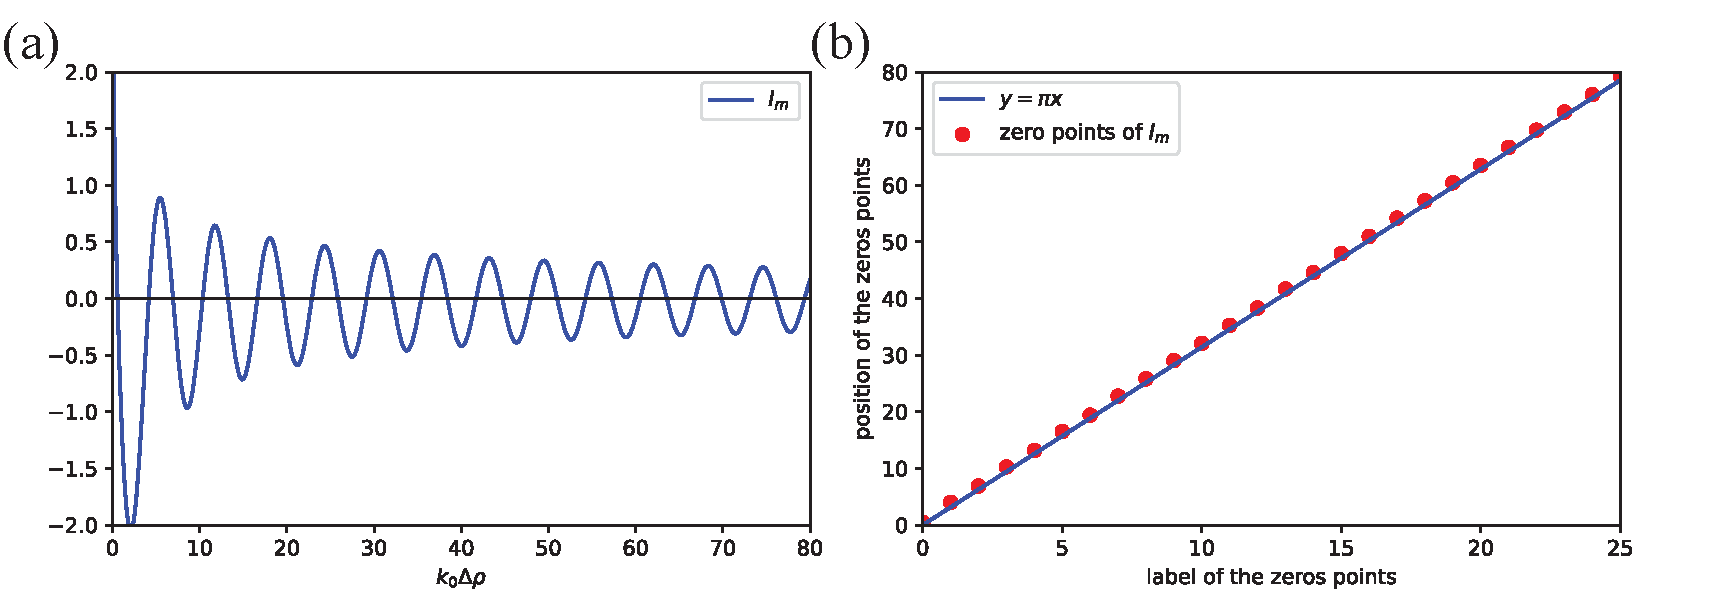
\includegraphics[width=  \linewidth]{SIfig/I_3.pdf}
\caption{
    Numerical results of~$I_{m}$ is shown in (a), and the position of the zero points are shown in (b).
}
\label{fig:I_3}
\end{figure}

\section{Particle-particle summation in long-range terms}

Here we deal with the particle-particle summation, which is a double summation and need~$N^2$ steps if being calculated directly.
In standard Ewald sum, its particle-particle summation is handle as
\begin{equation}\label{eq:sum_direct}
    \sum_{i, j} q_i q_j cos(\V{k} \cdot \V{r}_{ij}) = \text{Re} \left[ \sum_i q_i e^{i \V{k} \V{r}_i} \right]^2\;,
\end{equation}
and then the double summation is reduced to a single one.
However, Eq.~\eqref{eq:U_l} contains following terms
\begin{equation}\label{eq:L}
\begin{split}
    L_1 &= \sum_{i, j} q_i q_j \abs{z_i - z_j}\;,\\
    L_2^{\pm} &= \sum_{i, j} q_i q_j e^{\pm k\abs{z_i - z_j}} \cos{(\V{k} \cdot \V{\rho}_{ij})}\;,\\
    L_3^{\pm} &= \sum_{i, j} q_i q_j e^{\pm k(z_i + z_j)} \cos{(\V{k} \cdot \V{\rho}_{ij})}\;,
\end{split}
\end{equation}
and only~$L_3$ can be directly handled by strategy in Eq.~\eqref{eq:sum_direct} via
\begin{equation}
    L_3 = \text{Re} \left[ \sum_{i = 1}^N q_i e^{\pm k z_i} e^{i \V{k} \cdot \V{\rho}} \right]^2\;,
\end{equation}
while~$L_1$ and~$L_2$ contains~$\abs{z_i \pm z_j}$ terms so that can not be calculated as~$L_3$.

To calculate~$L_1$ and~$L_2$, we apply some new strategy by using idea of bucket sort method.
Notice that to simplify calculation of~$L_1$ and~$L_2$, the difficulty rise from the unknown sign of~$\abs{z_i - z_j}$, so it is nature to consider that we may sort all~$z_i$ up so that
\begin{equation}
    0 < z_1 < ... < z_i < ...  < z_N < L_z\;.
\end{equation}
where we use the idea of bucket sort algorithm to fasten the sorting because the upper and lower bound of~$z_i$ are definite.
For that purpose, we build a~$N$-cell list in~$z$, and then use merge sort to sort elements in each cell. 
Because average element number in each cell is simply~$1$, complexity of sorting will be
\begin{equation}
    N_{\text{sort}} \sim \sum_{i = 1}^{N} \mathcal{O}(n_i \log n_i) \sim N \times \mathcal{O}(\bar{n} \log \bar{n}) \sim \mathcal{O}(N)\;.
\end{equation}

Then, for~$L_1$, we can write it as
\begin{equation}
\begin{split}\label{eq:L_1}
    L_1 & = \sum_{i = 1}^{N} q_i \left[ - \sum_{j = 1}^{j = i} q_j (z_i - z_j) + \sum_{j = i+1}^{j = N} q_j (z_i - z_j) \right] \\
    & = 2 \sum_{i = 1}^{N} q_i z_i \left[ - \sum_{j = 1}^{j = i}q_j + \sum_{j = i+1}^{j = N} q_j \right] = 4 \sum_{i = 1}^{N} q_i z_i A_i \;,
\end{split}
\end{equation}
where~$A_i = - \sum_{j = 1}^{j = i}q_j$, and can be calculated by iterative method, i.e.
\begin{equation}\label{eq:A}
    A_1 = - q_1,~A_{i + 1} = A_i - q_{i + 1}\;.
\end{equation}
In this way, generating array~$A$ takes~$N$ steps, an then calculating the summation in Eq.~\eqref{eq:L_1} will take another~$2N$ steps.

For calculation of~$L_2$, the idea is similar.
First, we can write~$L_2^+$ as
\begin{equation}
\begin{split}
    L_2^+  & = \sum_{i, j} q_i q_j e^{ k\abs{z_i - z_j}} \cos{(k_x (x_i - x_j) + k_y (y_i - y_j))}\\
    & = \sum_{i, j} e^{ k\abs{z_i - z_j}} \left[ c_i c_j - s_i s_j \right]\;,
\end{split}
\end{equation}
where~$c_i = q_i \cos{(k_x x_i + k_y y _i)}$ and~$s_i = q_i \sin{(k_x x_i + k_y y _i)}$.
Then using the sorted~$z_i$, we can write
\begin{equation}\label{eq:L_2_sum}
    \begin{split}
    \sum_{i, j} c_i c_j e^{ k\abs{z_i - z_j}} = 2 \sum_{i = 1}^{N} c_i e^{k z_i} \sum_{j = 1}^{i} c_j e^{ - k z_j} = 2 \sum_{i = 1}^{N} c_i e^{k z_i} C_i\;,\\
    \sum_{i, j} s_i s_j e^{ k\abs{z_i - z_j}} = 2 \sum_{i = 1}^{N} s_i e^{k z_i} \sum_{j = 1}^{i} s_j e^{ - k z_j} = 2 \sum_{i = 1}^{N} s_i e^{k z_i} S_i\;,
\end{split}
\end{equation}
where~$C_i = \sum_{j = 1}^{i} c_j e^{ - k z_j}$ and~$S_i = \sum_{j = 1}^{i} s_j e^{ - k z_j}$, which can also be calculated by iterative method, i.e.
\begin{align}
    C_1 = 0,~C_{i + 1} = C_i + c_{i + 1} e^{ - k z_{i + 1}}\;, \label{eq:C}\\
    S_1 = 0,~S_{i + 1} = S_i + s_{i + 1} e^{ - k z_{i + 1}}\;. \label{eq:S}
\end{align}
Then generating array~$C$ and~$S$ takes~$2N$ steps, and summations in Eq.~\eqref{eq:L_2_sum} cost another~$4N$ steps.

\section{Algorithm and time complexity}

According to discussions above, our algorithm is given by Algorithm~\ref{alg:QEM_nrbm}.
The time complexity of computing long-range and short-range interaction then is given by
\begin{equation}
    \begin{split}
        C_s & = S_r \times \rho_r \times N = N \times \frac{N}{L_x L_y} \times \pi r_c^2  = \frac{\pi N^2 s^2}{L_x L_y \alpha}\;,\\
        C_l &= S_k \times \rho_k \times N = \pi k_c^2 \times \frac{L_x L_y}{4 \pi^2} \times N = \frac{L_x L_y N s^2 \alpha}{\pi}\;,
    \end{split}
\end{equation}
where $\rho_r$, $\rho_k$ for density in real and reciprocal space. To balance complexity, we take 
\begin{equation}
    \alpha = \frac{\sqrt{N}}{L_x L_y}\;,
\end{equation}
so that the total complexity is given by
\begin{equation}
    C = \pi s^2 N^{1.5} + \pi^{-1} s^2 N^{1.5} \sim O(N^{1.5})\;,
\end{equation}
which is one of the fast among all algorithm handling dielectric confined quasi-2D charged systems.

\begin{algorithm}
\caption{Quasi-Ewald method}
\label{alg:QEM_nrbm}
\begin{algorithmic}
\STATE{Choose~$r_c$,~$k_c$ and~$t$.}
\STATE{Using position of particles, build up cell lists in~$xy$ and $z$.}
\FOR{i in 1:~$N$}
    \STATE{Determine particles as neighbor of particle~$i$, and form a set~$N_{\text{near}}$.}
    \FOR{j in 1:~$N_{\text{near}}$}
        \STATE{Calculate numerical solution of Eq.~\eqref{eq:G_1_int} to get short range interaction between~$i$ and~$j$.}
        \STATE{Short range interaction energy added by~$U_{s, ij}$.}
    \ENDFOR
\ENDFOR
\STATE{Sort~$z_i$ in each cells.}
\FOR{$\abs{\V{k}} < k_c$}
    \FOR{i in $1:N$}
       \STATE{Generate~$A_i$,~$C^{\pm}_i$ and~$S^{\pm}_i$ using iterative method as given in Eq.~\eqref{eq:A},~\eqref{eq:C} and~\eqref{eq:S}.}
    \ENDFOR
    \STATE{Calculate~$L_1$,~$L_2^\pm$ and~$L_3^\pm$ defined in Eq.~\eqref{eq:L} using array~$A$,~$C$ and~$S$.}
    \STATE{Calculate long range interaction energy corresponding to~$\V{k}$.}
    \STATE{Long range interaction energy added by~$U_{l,\V{k}}$.}
\ENDFOR
\RETURN{$U = U_l + U_s$}
\end{algorithmic}
\end{algorithm}


% And for the integral over~$g_2(k, z, z_s)$, using the fact that
% \begin{equation}
%     \int_0^{\infty} e^{- k a}J_0(k \rho) dk = \frac{1}{\sqrt{a^2 + \rho^2}}\;,
% \end{equation}
% so that it can be given analytically as
% \begin{equation}
%     - \int_{0}^{+\infty} \frac{1}{2} \sum_{l = 1}^{4} \Gamma_l e^{-k a_l} J_0(k \Delta \rho) d k = - \sum_{l = 1}^{4} \frac{\Gamma_l}{2 \sqrt{a_l^2 + \Delta \rho^2}}\;.
% \end{equation}

% For $I_2$, there is no need to use strategy in Eq.~\eqref{eq:beta_split} because its integrand is coupled with the fast decaying term~$e^{-\frac{k^2}{4 \alpha}}$.
% The process is similar to that of calculating~$I_1$, and the error of evaluating the infinite integral is proportional to
% \begin{equation}
%     \Delta_2 \propto \abs{\int_{k_f}^{+\infty} \frac{\sum_{l = 1}^{4} \Gamma_l e^{-k a_l - k^2 / (4 \alpha)} J_0(k \Delta \rho)}{\gamma_1 \gamma_2 e^{-2k L_z} - 1}   \text{d} k} < \int_{k_f}^{+\infty} \sum_{l = 1}^{4} \abs{\Gamma_l} \beta^{-1} e^{ - k^2 / (4 \alpha)} \text{d} k = \chi_2 \mathrm{erfc}\left(\frac{k_{f}}{2 \alpha}\right)\;.
% \end{equation}

% Using these methods,~$G_1(k, z, z_s)$ is properly handled.

% where~$\beta_1(k) \to -\frac{(\eps - \eps')^2}{(\eps + \eps')^4}$ as~$k \to \infty$, which can be treated as a constant (except for $\eps + \eps' = 0$ in which case the problem is ill-defined and non-physical).
% Then Eq.~\eqref{eq:gkz_expresson} can be split into two terms, i.e.
% \begin{equation}
%     g(k, z;z^\prime) = \frac{1}{2k} \sum_{i = 1}^{4} \big[ \beta_1(k) \Gamma_i e^{k (a_i - 2 L_z)} + \beta_2 \Gamma_i e^{k a_i} \big]\;,
% \end{equation}
% further use the fact that
% \begin{equation}
%     \int_0^{\infty} e^{k a}J_0(k \rho) dk = \frac{1}{\sqrt{a^2 + \rho^2}}\;,
% \end{equation}
% Eq.~\eqref{eq:phi_1} can be re-written as
% \begin{align}
%     G_1(\V{r};~\V{r^\prime})
%     = & - \frac{1}{4 \pi \eps} \sum_{\V{m}} \sum_{i = 1}^{4} \int_{0}^{+\infty}  \big[ \beta_1(k) \Gamma_i e^{k (a_i - 2 L_z)} + \beta_2 \Gamma_i e^{k a_i} \big] (1-e^{-\frac{\V{k}^2}{4 \alpha}}) J_0(k \abs{\V{\rho} - \V{\rho^\prime_m}})  d k \notag\\
%     = & \frac{1}{4 \pi \eps} \sum_{\V{m}} \sum_{i = 1}^{4} \int_{0}^{+\infty}  \big[ \beta_1(k) \Gamma_i e^{k (a_i - 2 L_z)} + \beta_2 \Gamma_i e^{k a_i} \big] e^{-\frac{\V{k}^2}{4 \alpha}} J_0(k \abs{\V{\rho} - \V{\rho^\prime_m}})  d k \label{eq:G_1_full} \\
%      & -  \int_{0}^{+\infty} \beta_1(k) \Gamma_i e^{k (a_i - 2 L_z)} J_0(k \abs{\V{\rho} - \V{\rho^\prime_m}}) d k -  \frac{\beta_2 \Gamma_i}{\sqrt{a_i^2 + \abs{\V{\rho} - \V{\rho^\prime_m}}^2}} \; \notag,
% \end{align}
% with the following expressions for coefficients $A_i$, $B_i$ and $C_i$:
% \begin{align}
%     A_i(k) & = \frac{1}{4 \pi \eps} \big[ \beta_1(k) \Gamma_i e^{- 2 L_z k} + \beta_2 \Gamma_i \big] \;,\\
%     B_i(k) & = - \frac{1}{4 \pi \eps} \beta_1(k) \Gamma_i \;, \\
%     C_i & = - \frac{1}{4 \pi \eps} \beta_2 \Gamma_i\;.
% \end{align}
% Clearly, all oscillatory terms due to $J_0$ are now multiplied by an exponentially decaying prefactor, and can be calculated with much less effort.

% For simplicity, the integrals involved in Eq.~\eqref{eq:G_1_full} can be reduced into the following two forms,
% \begin{align}
%     I_1 & = \int_0^{\infty} f_1(k) \mathrm{e}^{-2 k L_z} J_0(k \rho) dk\;, \label{eq:int_1}\\ 
%     I_2 & = \int_0^{\infty} f_2(k) \mathrm{e}^{- k^2 / 4 \alpha} J_0(k \rho) dk\;. \label{eq:int_2} 
% \end{align}
% Usually, the integrals in Eq.~\eqref{eq:int_1} and~\eqref{eq:int_2} can be calculated by Gauss–Laguerre quadrature and Gauss–Hermite quadrature, respectively.
% %i.e.
% %\begin{align}
% %    I = \sum_{i = 1}^{n} \omega_i F(x_i)\;, \label{eq:discrete}
% %\end{align}
% %where~$\omega_i$ and~$x_i$ are weights and nodes from Gauss–Laguerre or Gauss–Hermite quadrature.
% However, recent work~\cite{trefethen2022exactness} shows that evaluating such improper integrals via truncating them onto finite domains~$(0,~k_f)$ actually will lead to a better accuracy when using the same number of sampling points, simply because the integral on~$(k_f, \infty)$ is negligible.
% So that for our case, by choosing proper cut-offs~$k_{f1}$ and~$k_{f2}$ for Eqs.~\eqref{eq:int_1} and Eq.~\eqref{eq:int_2}, we can truncate these improper integrals onto finite domains, and evaluate the definite integrals using Gauss quadrature.

% Furthermore, we obtain the following upper bound for the truncation error:
% \begin{align}
%     \Delta I_1 &= \abs{\int_{k_{f1}}^{\infty} f(k) \mathrm{e}^{-2 k L_z} J_0(k \rho) dk} < \int_{k_{f1}}^{\infty} \max{(\abs{f_1(k)})} \mathrm{e}^{-2 k L_z} \frac{1}{\sqrt{k \rho}} dk = \chi_1 \mathrm{erfc}\left(\sqrt{2 k_{f1} L_z}\right)\;,\\
%     \Delta I_2 &= \abs{\int_{k_{f2}}^{\infty} g(k) \mathrm{e}^{- k^2 / 4 \alpha} J_0(k \rho) dk} < \int_{k_{f2}}^{\infty} \max{(\abs{f_2(k)})} \mathrm{e}^{- k^2 / 4 \alpha}  dk = \chi_2 \mathrm{erfc}\left(\frac{k_{f2}}{2 \alpha}\right)\;,
% \end{align}
% where~$\chi_i$ are constants. Clearly, the truncation error is controlled by $\mathrm{erfc(\cdot)}$ which vanishes rapidly. 
% Thus for the truncated integral we can simply use Gauss–Legendre quadrature to obtain highly accurate results, hence the difficulties caused by the oscillatory and slow decaying Bessel function $J_0$ is resolved.



\section{Numerical Validations}
% To validate our method (in what follows, our method is denoted as QEM, namely Quasi-Ewald Method), we compare our force calculation results against ICM.
% Using the same setup as in main text, we calculate the force in~$x$ direction between two cations with valence~$+1$ as shown in Fig.~\ref{fig:ICM-QEM}.
% For both~$\gamma = 0.95$ and~$\gamma = -0.95$, the discrepancy between QEM and ICM is less than 1E-3, which validates our method. Note that ICM needs~$\sim8000$ image charges to reach 3-4 digit accuracy due to the slow convergence of image reflection series, the QEM is much more efficient.

% \begin{figure}[htbp]
% 	\centering
% 	\includegraphics[width=0.5\textwidth]{../Symmetry Breaking/SIfig/SI1.pdf}
% 	\caption{Force between two particles with charge $e_0$ in a quasi-2D system of size~$(30\tau_0,~30\tau_0,~2\tau_0)$, and the medium's Bjerrum length~$l_B = 3.5 \tau_0$. 
% 	Particles are placed at $(15\tau_0,~15\tau_0,~\tau_0)$ and~$(15\tau_0 + \Delta x,~15\tau_0,~\tau_0)$. 
% 	Solid lines are resultes obtained via QEM, dots via ICM.
% 		\label{fig:ICM-QEM}
% 	}
% \end{figure}

We validate our method (in what follows, our method is denoted as QEM, namely Quasi-Ewald Method) in MD simulations via cross comparing with recent simulation results.
Using the same reduced units as defined in main text, we test cases the system with parameters~$L_x = L_y = 100 \tau_0$, $L_z = 50 \tau_0$,~$\gamma = \pm 0.95$, $T_r=1$, and number of cations and anions are both~$218$.
For both cases it costs $6 \times 10^5$ time steps to reach equilibrium, after which we continue the simulation for $4 \times 10^5$ time steps for sampling.
The calculated ion density profiles are shown in Fig.~\ref{fig:QEM_HSMA}, which clearly maintains all symmetry properties of the system, and is consistent with results reported in Refs.~\cite{liang2020harmonic,yuan2021particle}.
\begin{figure}[htbp]
	\centering
	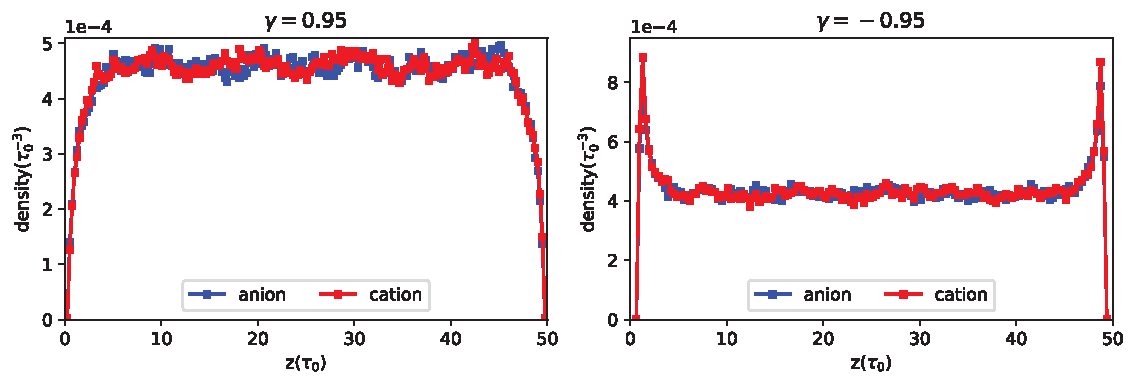
\includegraphics[width=0.6\textwidth]{SIfig/MD_simple.pdf}
	\caption{
	Distributions of ion density for symmetric electrolytes confined by neutral dielectric substrates, with $\gamma = \pm 0.95$.
		\label{fig:QEM_HSMA}
	}
\end{figure}

% \section{Relation between Resonance frequency and wavelength of SSPWs}

% As mentioned in the main text, we demonstrate that there is a simple relation between the resonance frequency~$k_0$ and the wavelength~$\lambda$ of static surface plasmonic waves, given by
% \begin{equation}
%     k_0 \cdot \lambda \sim 2 \pi\;.
% \end{equation}
% Some semi-quantitative proofs have already given in main text, and here some numerical results are shown in Fig.~\ref{fig:k_wavelegth}.

% \begin{figure}[htbp]
%     \centering
%     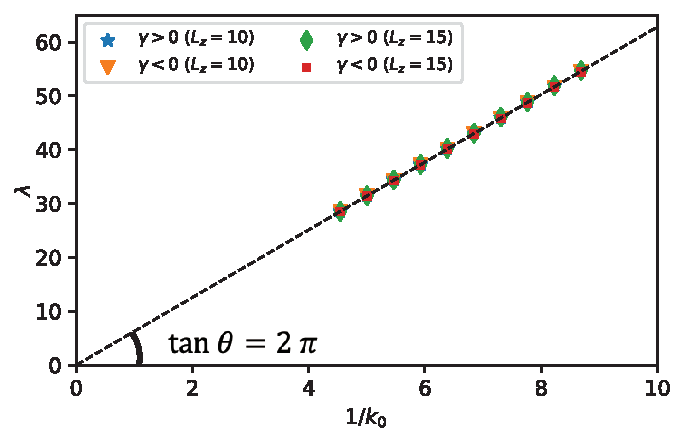
\includegraphics{SIfig/k_wavelegth.pdf}
%     \caption{Numerical results for relation between~$k_0$ and~$\lambda$}
%     \label{fig:k_wavelegth}
% \end{figure}


% We take different~$L_z$, i.e.~$10$ and~$15$, and then change the value of~$\gamma$ to tune~$k_0$.
% For each point, we randomly generated~$z$ and~$z_s$ as the position of the source charge and the test charge, respectively. Then we move the test charge along~$x$ axis, and take an average on distance between zeros points of~$E_x$.
% The numerical results show that the relation is highly robust and has no relation to position of the ions.

\section{Details of MD results}

In main text, we have shown that the charge oscillation can lead to lattice-like structure formation in dielectric confined quasi-2D systems, and mainly focused on the tunable lattice parameter.
Here we will discuss more about our results.

\begin{figure}[htbp]
    \centering
    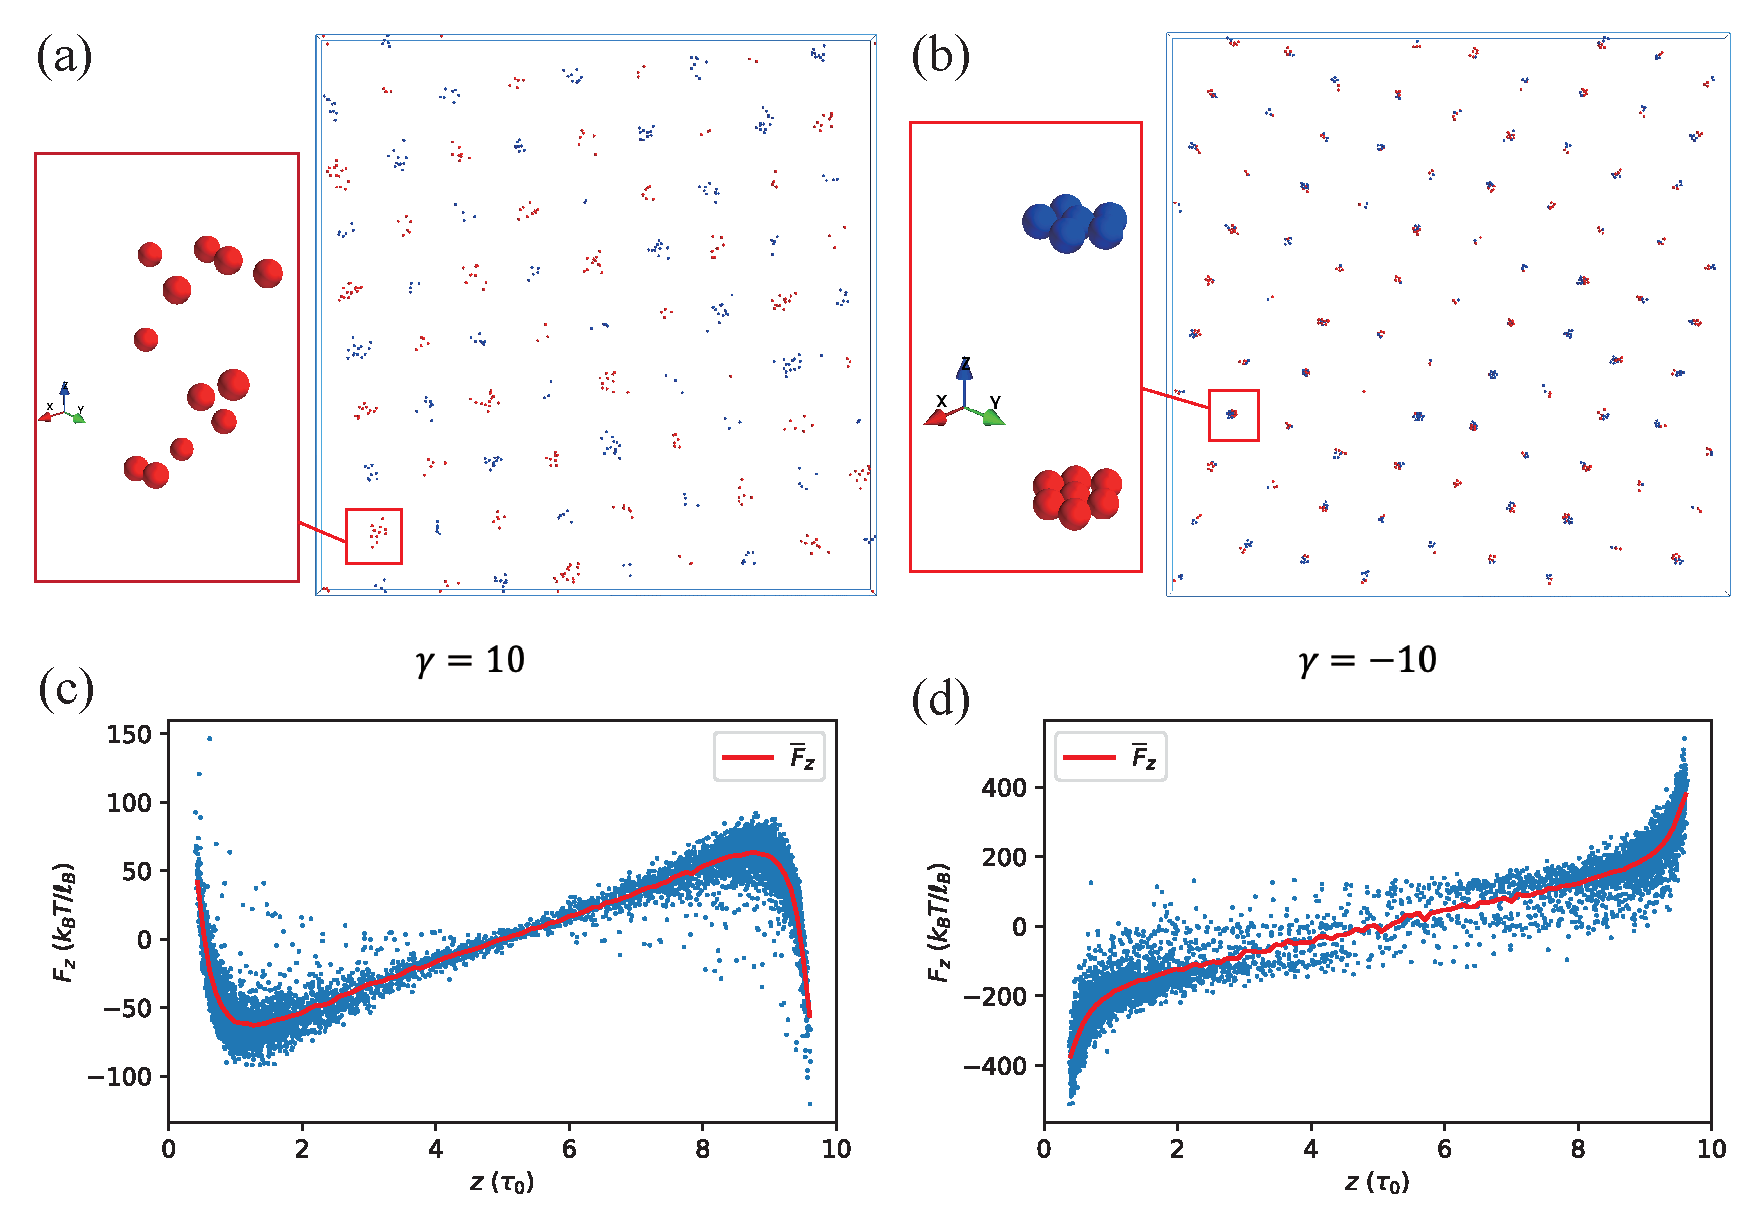
\includegraphics[width = \linewidth]{SIfig/MD_ball.pdf}
    \caption{The lattice-like structure and the cluster for~$\gamma = \pm 10$ cases are shown in (a) and (b), respectively. Force in~$z$ direction on particles at different position are shown in (b).}
    \label{fig:balls}
\end{figure}

As shown in Fig.~\ref{fig:balls} (a) and (b), the ions distribute near the substrates and pair with other ions on the opposite side.
For~$\gamma = 10$ and~$-10$ cases, the pairs are symmetric and anti-symmetric, respectively, as shown in the sub-figure.
The difference come from the sign of the reflection rate, which determines whether the polarized charges at opposite positions are of the same sign or of different sign, thus determines the symmetry of the ions on the opposite sites.

Shapes of the clusters are also different.
For both cases, we attribute the cluster formation to the strong polarization charge with different sign on the substrate as shown in Fig.~1~(a) of the main text, which form a deep potential well and trapped these ions inside.
In the transverse direction, when~$\gamma = 10$, the ions forms ion liquid and separate from each other, and when~$\gamma = -10$, the ions are closely packed, because of the force in transverse direction between ions with the same sign are repulsive or attractive in short range, respectively.
In the vertical direction, we calculated force in~$z$ to explain the distribution in~$z$, as shown in Fig.~\ref{fig:balls} (c) and (d).
When~$\gamma = 10$, we found that the surface with opposite sign reverse the force in the middle region and pull the ions to the substrates, so that the ions are distributed near the substrates but not attached to them.
When~$\gamma = -10$, the force is purely attractive and the ions are all attached to the substrates.




\bibliography{SSBbib}


% \begin{thebibliography}{3}%
% 	\makeatletter
% 	\providecommand \@ifxundefined [1]{%
% 		\@ifx{#1\undefined}
% 	}%
% 	\providecommand \@ifnum [1]{%
% 		\ifnum #1\expandafter \@firstoftwo
% 		\else \expandafter \@secondoftwo
% 		\fi
% 	}%
% 	\providecommand \@ifx [1]{%
% 		\ifx #1\expandafter \@firstoftwo
% 		\else \expandafter \@secondoftwo
% 		\fi
% 	}%
% 	\providecommand \natexlab [1]{#1}%
% 	\providecommand \enquote  [1]{``#1''}%
% 	\providecommand \bibnamefont  [1]{#1}%
% 	\providecommand \bibfnamefont [1]{#1}%
% 	\providecommand \citenamefont [1]{#1}%
% 	\providecommand \href@noop [0]{\@secondoftwo}%
% 	\providecommand \href [0]{\begingroup \@sanitize@url \@href}%
% 	\providecommand \@href[1]{\@@startlink{#1}\@@href}%
% 	\providecommand \@@href[1]{\endgroup#1\@@endlink}%
% 	\providecommand \@sanitize@url [0]{\catcode `\\12\catcode `\$12\catcode
% 		`\&12\catcode `\#12\catcode `\^12\catcode `\_12\catcode `\%12\relax}%
% 	\providecommand \@@startlink[1]{}%
% 	\providecommand \@@endlink[0]{}%
% 	\providecommand \url  [0]{\begingroup\@sanitize@url \@url }%
% 	\providecommand \@url [1]{\endgroup\@href {#1}{\urlprefix }}%
% 	\providecommand \urlprefix  [0]{URL }%
% 	\providecommand \Eprint [0]{\href }%
% 	\providecommand \doibase [0]{https://doi.org/}%
% 	\providecommand \selectlanguage [0]{\@gobble}%
% 	\providecommand \bibinfo  [0]{\@secondoftwo}%
% 	\providecommand \bibfield  [0]{\@secondoftwo}%
% 	\providecommand \translation [1]{[#1]}%
% 	\providecommand \BibitemOpen [0]{}%
% 	\providecommand \bibitemStop [0]{}%
% 	\providecommand \bibitemNoStop [0]{.\EOS\space}%
% 	\providecommand \EOS [0]{\spacefactor3000\relax}%
% 	\providecommand \BibitemShut  [1]{\csname bibitem#1\endcsname}%
% 	\let\auto@bib@innerbib\@empty
% 	%</preamble>
% 	\bibitem [{\citenamefont {Trefethen}(2022)}]{trefethen2022exactness}%
% 	\BibitemOpen
% 	\bibfield  {author} {\bibinfo {author} {\bibfnamefont {L.~N.}\ \bibnamefont
% 			{Trefethen}},\ }\bibfield  {title} {\bibinfo {title} {Exactness of
% 			{Q}uadrature {F}ormulas},\ }\href {https://doi.org/10.1137/20M1389522}
% 	{\bibfield  {journal} {\bibinfo  {journal} {SIAM Rev.}\ }\textbf {\bibinfo
% 			{volume} {64}},\ \bibinfo {pages} {132} (\bibinfo {year} {2022})}\BibitemShut
% 	{NoStop}%
% 	\bibitem [{\citenamefont {Liang}\ \emph {et~al.}(2020)\citenamefont {Liang},
% 		\citenamefont {Yuan}, \citenamefont {Luijten},\ and\ \citenamefont
% 		{Xu}}]{liang2020harmonic}%
% 	\BibitemOpen
% 	\bibfield  {author} {\bibinfo {author} {\bibfnamefont {J.}~\bibnamefont
% 			{Liang}}, \bibinfo {author} {\bibfnamefont {J.}~\bibnamefont {Yuan}},
% 		\bibinfo {author} {\bibfnamefont {E.}~\bibnamefont {Luijten}},\ and\ \bibinfo
% 		{author} {\bibfnamefont {Z.}~\bibnamefont {Xu}},\ }\bibfield  {title}
% 	{\bibinfo {title} {Harmonic surface mapping algorithm for molecular dynamics
% 			simulations of particle systems with planar dielectric interfaces},\ }\href
% 	{https://doi.org/10.1063/5.0003293} {\bibfield  {journal} {\bibinfo
% 			{journal} {J. Chem. Phys.}\ }\textbf {\bibinfo {volume} {152}},\ \bibinfo
% 		{pages} {134109} (\bibinfo {year} {2020})}\BibitemShut {NoStop}%
% 	\bibitem [{\citenamefont {Yuan}\ \emph {et~al.}(2021)\citenamefont {Yuan},
% 		\citenamefont {Antila},\ and\ \citenamefont {Luijten}}]{yuan2021particle}%
% 	\BibitemOpen
% 	\bibfield  {author} {\bibinfo {author} {\bibfnamefont {J.}~\bibnamefont
% 			{Yuan}}, \bibinfo {author} {\bibfnamefont {H.~S.}\ \bibnamefont {Antila}},\
% 		and\ \bibinfo {author} {\bibfnamefont {E.}~\bibnamefont {Luijten}},\
% 	}\bibfield  {title} {\bibinfo {title} {Particle--{p}article
% 			{p}article--{m}esh algorithm for electrolytes between charged dielectric
% 			interfaces},\ }\href {https://doi.org/10.1063/5.0035944} {\bibfield
% 		{journal} {\bibinfo  {journal} {J. Chem. Phys.}\ }\textbf {\bibinfo {volume}
% 			{154}},\ \bibinfo {pages} {094115} (\bibinfo {year} {2021})}\BibitemShut
% 	{NoStop}%
% \end{thebibliography}%

\end{document}

